\documentclass{standalone}
\usepackage{tikz}
\usetikzlibrary{decorations.pathmorphing}

\begin{document}
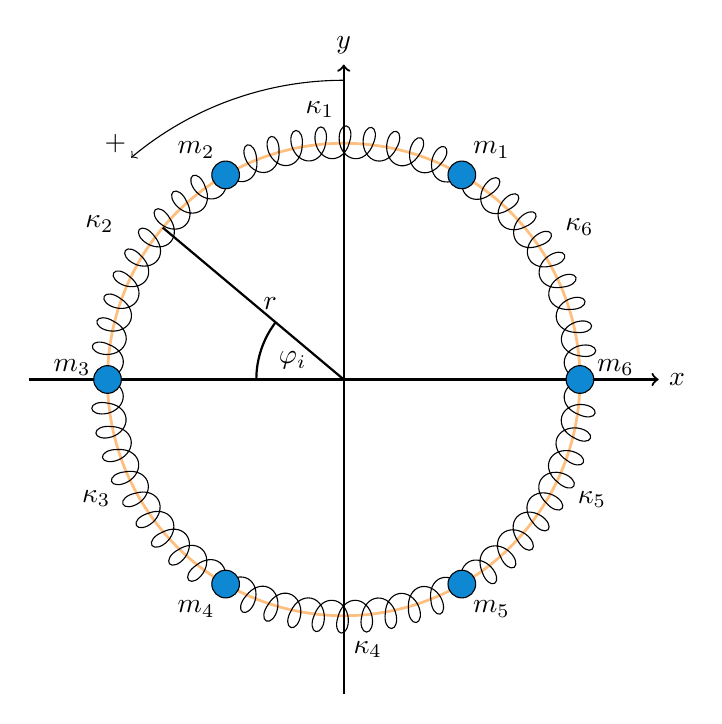
\begin{tikzpicture}
    % Define the radius of the circle
    \def\radius{3}
    % Define a new length for r
    \def\rLength{3}  % Adjust this value to change the length of r

    % Draw the perimeter of the circle with opacity
    \draw[orange, line width=1pt, opacity=0.5] (0, 0) circle (\radius);  % Circle outline with opacity
    
    % Draw the circular springs (coils) between masses using the decorate package (in black)
    \draw[thin, color=black, decoration={coil, aspect=0.7, segment length=3mm, amplitude=2mm}, decorate] 
        (0:\radius) arc[start angle=0, end angle=60, radius=\radius] node[midway, above left, xshift=0.70cm, yshift=0.21cm] {$\kappa_6$}; 
    \draw[thin, color=black, decoration={coil, aspect=0.7, segment length=3mm, amplitude=2mm}, decorate] 
        (60:\radius) arc[start angle=60, end angle=120, radius=\radius] node[midway, above left, yshift=0.2cm] {$\kappa_1$}; 
    \draw[thin, color=black, decoration={coil, aspect=0.7, segment length=3mm, amplitude=2mm}, decorate] 
        (120:\radius) arc[start angle=120, end angle=180, radius=\radius] node[midway, below left, xshift=-0.20cm, yshift=0.70cm] {$\kappa_2$}; 
    \draw[thin, color=black, decoration={coil, aspect=0.7, segment length=3mm, amplitude=2mm}, decorate] 
        (180:\radius) arc[start angle=180, end angle=240, radius=\radius] node[midway, below right, xshift=-0.85cm, yshift=0.21cm] {$\kappa_3$}; 
    \draw[thin, color=black, decoration={coil, aspect=0.7, segment length=3mm, amplitude=2mm}, decorate] 
        (240:\radius) arc[start angle=240, end angle=300, radius=\radius] node[midway, below right, yshift=-0.2cm] {$\kappa_4$}; 
    \draw[thin, color=black, decoration={coil, aspect=0.7, segment length=3mm, amplitude=2mm}, decorate] 
        (300:\radius) arc[start angle=300, end angle=360, radius=\radius] node[midway, above right, xshift=0.25cm, yshift=-0.25cm] {$\kappa_5$}; 

    % Add coordinate axes
    \draw[thick,->] (-4, 0) -- (4, 0) node[right] {$x$}; % x-axis label
    \draw[thick,->] (0, -4) -- (0, 4) node[above] {$y$}; % y-axis label

    % Draw radial and angular parameters (r and phi_j)
    \draw[-, black, thick] (0,0) -- ({\rLength*cos(140)},{\rLength*sin(140)}) node[midway, right, black] {$r$}; % Adjust length and angle of r
    \path [->, green, thick] (0:\radius) arc (0:60:\radius);

    % Draw the arc with an arrow from the y label to the II quadrant, increased size
    \draw[->, thin] (0, 3.8) arc[start angle=90, end angle=130, radius=4.2cm];
    \draw[-, thick] (-1.11, 0) arc[start angle=180, end angle=143, radius=1.2cm];
    \node at (-0.65,0.24) {$\varphi_i$};
    % Add the "+" label to the arc
    \node at (-2.9, 3) {$+$}; % Position of the label

    % Draw the six masses with manual positioning for m_i labels
    \foreach \i in {1, 2, 3, 4, 5, 6} {
        % Place the masses at equal angles (60 degrees apart)
        \node[draw, circle, fill=cyan!70!blue, minimum size=10pt, inner sep=0pt] (m\i) at ({\i*60}:\radius) {};  % Smaller size
        % Adjust label positions manually
        \ifnum\i=1
            \node[xshift=0.25cm, yshift=0.1cm] at ({\i*60}:\radius + 0.25) {$m_\i$};  % Adjusted m1 position
        \else\ifnum\i=2
            \node[xshift=-0.25cm, yshift=0.1cm] at ({\i*60}:\radius + 0.25) {$m_\i$};  % Adjusted m2 position
        \else\ifnum\i=3
            \node[xshift=-0.20cm, yshift=0.15cm] at ({\i*60}:\radius + 0.25) {$m_\i$};  % Adjusted m3 position
        \else\ifnum\i=4
            \node[xshift=-0.25cm, yshift=-0.1cm] at ({\i*60}:\radius + 0.25) {$m_\i$};  % Adjusted m4 position
        \else\ifnum\i=5
            \node[xshift=0.25cm, yshift=-0.1cm] at ({\i*60}:\radius + 0.25) {$m_\i$};  % Adjusted m5 position
        \else\ifnum\i=6
            \node[xshift=0.20cm, yshift=0.15cm] at ({\i*60}:\radius + 0.25) {$m_\i$};  % Adjusted m6 position
        \fi\fi\fi\fi\fi\fi
    }

\end{tikzpicture}
\end{document}
